\documentclass[letterpaper,11pt]{amsart}

\usepackage{amscd,amssymb,amsfonts,amsmath,amsthm,color}
\usepackage{enumerate}
\usepackage{listings}
\usepackage{courier}
\usepackage{graphicx}
\usepackage{scrextend}

\usepackage{calc}
\newsavebox\CBox
\newcommand\hcancel[2][0.5pt]{%
  \ifmmode\sbox\CBox{$#2$}\else\sbox\CBox{#2}\fi%
  \makebox[0pt][l]{\usebox\CBox}%  
  \rule[0.5\ht\CBox-#1/2]{\wd\CBox}{#1}}


\lstset{frame=lrbt,xleftmargin=\fboxsep,xrightmargin=-\fboxsep,colframe=gray}


\lstset{basicstyle=\ttfamily\footnotesize,breaklines=true}


%%%%%%%%%%%%%%%%%%%%%%%%%%%%%%%%%%%%%%%%%%%%%%%%%%%%%%%%%%%%
% margins and style
\pagestyle{plain}
\setlength{\evensidemargin}{0.25in}
\setlength{\oddsidemargin}{0.25in}
\setlength{\textwidth}{6.0in}
\setlength{\topmargin}{0.0in}
\setlength{\textheight}{8.5in}
\setlength{\headheight}{0in}
\setlength{\parskip}{1.5mm}

\linespread{1.2}
\usepackage{color}
\definecolor{gray}{rgb}{0.3,0.3,0.3}



%%%%%%%%%%%%%%%%%%%%%%%%%%%%%%%%%%%%%%%%%%%%%%%%%%%%%%%%%%%%
% theorems and all 
\theoremstyle{plain}
\newtheorem{theorem}{Theorem}[section]
\newtheorem{lemma}[theorem]{Lemma}
\newtheorem{proposition}[theorem]{Proposition}
\newtheorem{corollary}[theorem]{Corollary}

\theoremstyle{definition}
\newtheorem{definition}[theorem]{Definition}
\newtheorem{remark}[theorem]{Remark}

%%%%%%%%%%%%%%%%%%%%%%%%%%%%%%%%%%%%%%%%%%%%%%%%%%%%%%%%%%%%
% renewed commands: t, to, d , c, H

%%%%%%%%%%%%%%%%%%%%%%%%%%%%%%%%%%%%%%%%%%%%%%%%%%%%%%%%%%%%
% Shortcuts for tex commands

\newcommand{\nc}{\newcommand}
\newcommand{\rc}{\renewcommand}
\nc{\mc}{\mathcal}
\rc{\t}{\text}
\nc{\loccit}{\emph{loc. cit. }}
\nc\pf{\noindent Proof: }
%%%%%%%%%%%%%%%%%%%%%%%%%%%%%%%%%%%%%%%%%%%%%%%%%%%%%%%%%%%%
% Operators, functions etc
\nc{\Hom}{\t{Hom}}
\nc{\tot}{\t{tot}}
\nc{\dual}{^{\vee}}
\nc{\op}[1]{\operatorname{#1}}
\nc{\coh}{\t{coh}}
\nc{\iso}{\cong}
\rc{\d}{\operatorname{d}}
\nc{\Id}{\operatorname{Id}}
\nc{\dgmod}{\operatorname{dg-mod}}
\newcommand{\hdot}{^{\raisebox{0pt}{\text{\circle*{2}}}}}
\nc{\compose}{\circ}
\nc{\sheafsym}{\mathcal{S}\t{ym}}
\nc{\rend}{\operatorname{REnd}}
\nc{\rhom}{\operatorname{RHom}}
\nc{\sheafrend}{\mathcal{R}\mc{E}\t{\emph{nd}}}
\nc{\sheafrhom}{\mathcal{R}\mc{H}\t{\emph{om}}}
\nc{\sheafhom}{\mathcal{H}\t{om}}
\nc{\exterior}{{\textstyle\bigwedge\nolimits}}
\nc{\ex}{\exterior}
\nc{\cok}{\operatorname{Coker}}
\rc{\ker}{\operatorname{Ker}}
\nc{\im}{\operatorname{Im}}

%tensor product
\nc{\Lotimes}{{\overset{L}{\otimes}}}
%%%%%%%%%%%%%%%%%%%%%%%%%%%%%%%%%%%%%%%%%%%%%%%%%%%%%%%%%%%%
% Arrows and signs
\rc{\to}{\rightarrow}
\nc{\ot}{\leftarrow}
\nc\xto[1]{\xrightarrow{#1}}
\nc{\too}{\longrightarrow}
\nc{\oot}{\longleftarrow}
\nc{\into}{\hookrightarrow}
\nc{\mapsinto}{\hookrightarrow}
%%%%%%%%%%%%%%%%%%%%%%%%%%%%%%%%%%%%%%%%%%%%%%%%%%%%%%%%%%%%
% Categories
\nc{\D}{\operatorname{D}}
\nc{\Dsg}{\D_{{sg}}}
\nc{\Db}{\D^{{b}}}
\nc{\Dbgr}{\Db_{{gr}}}
\nc{\Dgr}{\D_{{gr}}}
\nc{\Dsggr}{\Dsg^{{gr}}}
\nc{\Cgr}{\operatorname{C}_{{gr}}}
\nc{\cCgr}{\cC_{gr}}
\nc{\cDgr}{\cD_{gr}}
\nc{\cDsggr}{\cD_{gr}^{sg}}
\nc{\cDbgr}{\cD_{gr}^{b}}
\nc{\cDsg}{\cD_{sg}}
\nc{\cDb}{\cD^{b}}
\rc{\H}{\operatorname{H}}

%%%%%%%%%%%%%%%%%%%%%%%%%%%%%%%%%%%%%%%%%%%%%%%%%%%%%%%%%%%%
% Nice letters
% cals
\nc{\cA}{\mc{A}}\nc{\cB}{\mc{B}}\nc{\cC}{\mc{C}}\nc{\cD}{\mc{D}}\nc{\cE}{\mc{E}}\nc{\cF}{\mc{F}}\nc{\cG}{\mc{G}}\nc{\cH}{\mc{H}}\nc{\cI}{\mc{I}}\nc{\cJ}{\mc{J}}\nc{\cK}{\mc{K}}\nc{\cL}{\mc{L}}\nc{\cM}{\mc{M}}\nc{\cN}{\mc{N}}\nc{\cO}{\mc{O}}\nc{\cP}{\mc{P}}\nc{\cQ}{\mc{Q}}\nc{\cR}{\mc{R}}\nc{\cS}{\mc{S}}\nc{\cT}{\mc{T}}\nc{\cU}{\mc{U}}\nc{\cV}{\mc{V}}\nc{\cW}{\mc{W}}\nc{\cX}{\mc{X}}\nc{\cY}{\mc{Y}}\nc{\cZ}{\mc{Z}}
% bbs
\nc{\PP}{\mathbb{P}}
\nc{\CC}{\mathbb{C}}
\nc{\ZZ}{\mathbb{Z}}
\nc{\HH}{\mathbb{H}}
\nc{\NN}{\mathbb{N}}
\nc{\QQ}{\mathbb{Q}}
\nc{\RR}{\mathbb{R}}


\nc{\code}[1]{{\texttt{#1}}}
\nc{\mcode}[1]{{\text{\texttt{#1}}}}



%%%%%%%%%%%%%%%%%%%%%%%%%%%%%%%%%%%%%%%%%%%%%%%%%%%%%%%%%%%%
% other useful commands
\let\oldmarginpar\marginpar
\renewcommand\marginpar[1]{\-\oldmarginpar[\raggedleft\footnotesize #1]%
{\raggedright\footnotesize #1}}
\nc\note[1]{\marginpar{#1}}

%%%%%%%%%%%%%%%%%%%%%%%%%%%%%%%%%%%%%%%%%%%%%%%%%%%%%%%%%%%%
%%%%%%%%%%%%%%%%%%%%%%%%%%%%%%%%%%%%%%%%%%%%%%%%%%%%%%%%%%%%
%%%%%%%%%%%%%%%%%%%%%%%%%%%%%%%%%%%%%%%%%%%%%%%%%%%%%%%%%%%%
%%%%%%%%%%%%%%%%%%%%%%%%%%%%%%%%%%%%%%%%%%%%%%%%%%%%%%%%%%%%
%%%%%%%%%%%%%%%%%%%%%%%%%%%%%%%%%%%%%%%%%%%%%%%%%%%%%%%%%%%%

\title{Homework 7}
\date{}
\begin{document}
\maketitle
\begin{center}
  \emph{Due Thursday, March 9, at 11pm}
  \vspace{0.3in}
  \end{center}


\noindent Please enter your answers into a Jupyter notebook and submit by the deadline via canvas. 

\subsection*{Monte-Carlo Estimation of $\pi$} Estimate $\pi$ by using the following method. Generate $N = 5000$ (or more) pairs of numbers that are each uniformly random in the interval $(0,1)$. Count the number of pairs that are within the circle defined by $x^2 + y^2 = 1$.
\begin{center}
\noindent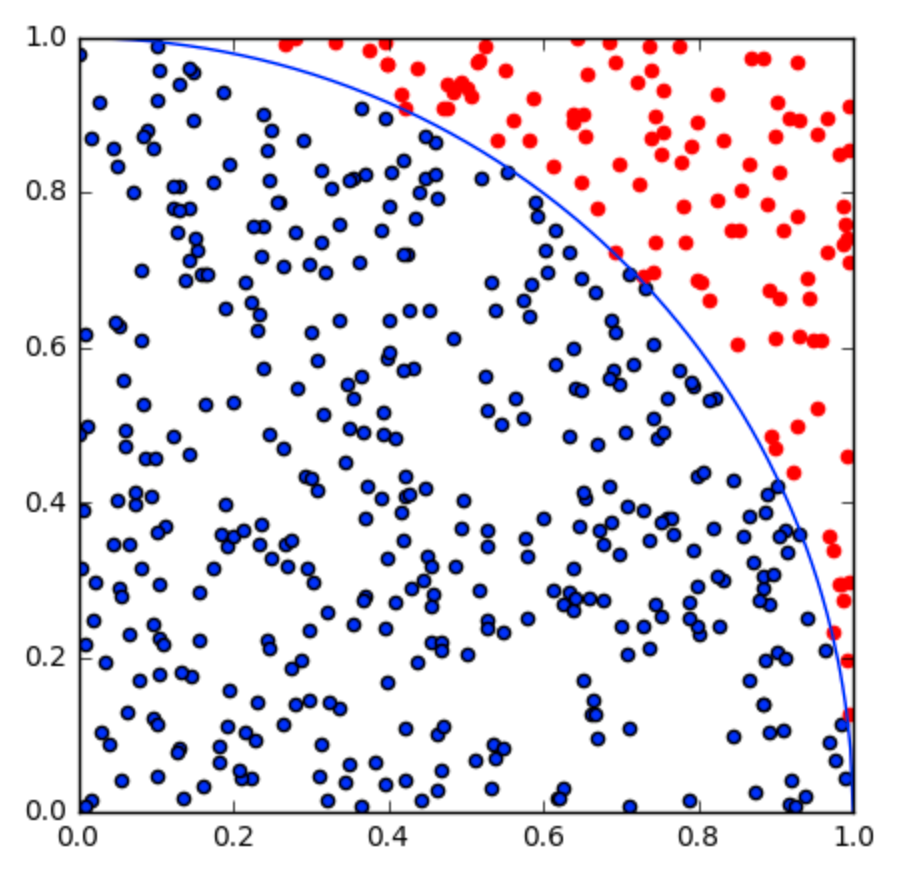
\includegraphics[width=2.6in]{monte_carlo.png}
\end{center}
Estimate $\pi$ this way and make the above plot using the code below:

\begin{lstlisting}[language=Python]
plt.figure(figsize=(5,5))
plt.scatter(X_out, Y_out, color="red")
plt.scatter(X_in,Y_in)
plt.plot(X, Y)
plt.axis([0, 1, 0, 1])
\end{lstlisting}

\subsection*{Random walks in two and three dimensions} In the last homework, we had the drunk bear Randi do a random walk in one dimension. We will now to the same in 2 and 3 dimensions. 
\begin{itemize}
  \item Imagine Randi is on a grid, at position $(0,0)$. At each time step, Randi goes, with equal probability, up, down, left or right (up means $y$ increases by 1 and right means $x$ increases by 1). Simulate 1000 random walks of length $m=1000,2000,\dots,10000$ in this 2-dimensional grid, and count the number of 2-dimensional random walks of Randi that end up with him going back to the origin at some point; and plot this as a function of $m$. Don't fill a giant numpy array with every simulation like we did in the last lecture (uses too much memory; instead, generate random walks one by one and store only the information you need).   
  \item Do the same in a three-dimensional grid (6 different directions for Randi to go at each step). 
\end{itemize}

As we discussed in class, this problem is about Polya's theorem. Which says that if you take a random walk in a 1 or 2-dimensional grid, then you will \emph{eventually} return to the starting position with probability 1 (i.e. the probability goes to 1 as $m$ goes to infinity). On the other hand, this is not true in 3 dimensions and above. For the 2D-random-walk plot you made, notice (mentally) how slowly the value goes to 1, whereas for the 3d version, it's not even close. 

\subsection*{Simulation of the Law of Large numbers and the Central Limit Theorem} We are drawing $n$ uniform random numbers. The average of these numbers will also be random but will have a different distribution. We want to see how the average changes (as a distribution) as $n$ increases.  

More precisely, let $x_1,x_2,x_2,\dots$ be drawn from the uniformly distribution between 0 and 1 (i.e. \code{random.random()}). Let 
$$y_n = \frac{x_1 + \dots + x_n}{n}$$ be the average. 

\begin{itemize}
  \item Write a function \code{get\_x()} that will return a uniformly random number between 0 and 1. 
  \item Write a function \code{get\_y(n)} that will return the average of $n$ random numbers picked by \code{get\_x()}. 
  \item (You can copy this from Lecture 20) Write a function \code{make\_hist(YY)} that will take a numpy array \code{YY}, make a histogram (use \code{normed=True} in \code{plt.hist(...)}) and plot the best fitting Gaussian curve to the content of YY. 
  \item For each of $n=1,10,100,1000,10000,100000$, sample 1000 values of $y_n$ (using \code{get\_y(n)}) and draw a histogram and the best fitting distribution. Print out the standard deviation of the data when $n=1$ (i.e. average of one single x; it should be 0.28). 
  \item For $n=1,2,\dots,100$, draw 1000 values from \code{get\_y()} and compute the standard deviation of the data (don't draw the histogram). Then plot the standard deviation value versus $n$. Also plot, in the same graph, the function $0.28 / \sqrt{n}$.
  \item Write briefly, why the results you got are consistent with the law of large numbers and the central limit theorem. 
\end{itemize}



\end{document}
%%%%%%%%%%%%%%%%%%%%%%%%%%%%%%%%%%%%%%%%%%%%%%%%%%%%%%%%%%%%






